\section{耦合传热传质的公共建模框架}

四个问题共用同一套守恒律、同一种边界条件形式和同一个求解器，差别只在物性库、求解区域与终止条件。本节一次性建立公共部分，各问章节只说明保留了什么、新增了什么以及结果因此改变了什么。

\subsection{几何降维与控制方程}

药材是一段长 25~cm、半径 2~cm 的圆柱。侧面积与两端面积之比等于长度与半径之比，端面只占总换热面积的 $7.4\%$，加之题目要求的结果都以“到药材中心的距离”标定，因此把三维圆柱问题降为一维径向问题。降维之后表面只剩一个环柱面，它同时承担对流换热与对流传质两个交换过程，轴线则由对称性给出零通量。图~\ref{fig:mech-geometry} 把这一降维过程与三处边界的类型画在一起。

\begin{figure}[htbp]
  \centering
  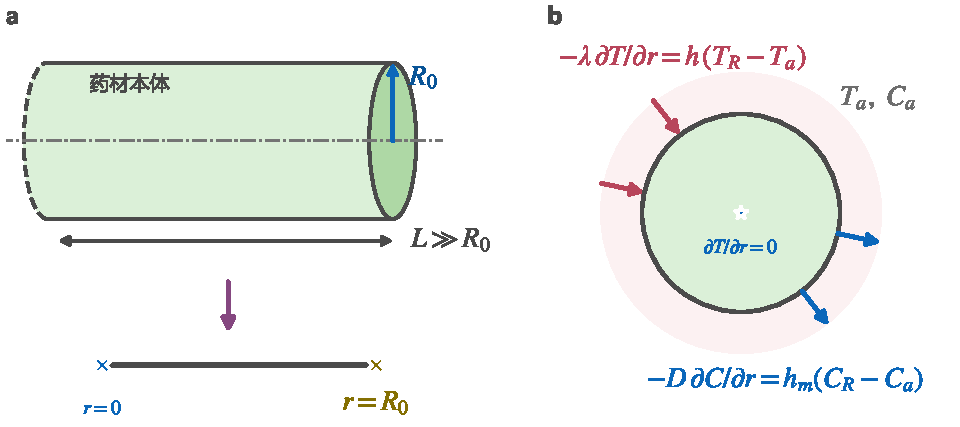
\includegraphics[width=0.9\textwidth,height=0.8\textheight,keepaspectratio]{../figures/fig_mech_geometry.pdf}
  \caption{几何降维与边界条件。长径比足够大时轴向与周向梯度可略，三维圆柱
  问题降为一维径向问题；表面同时承担对流换热与对流传质两个 Robin 条件，
  轴线处由对称性给出零通量。}
  \label{fig:mech-geometry}
\end{figure}

图中表面处两个箭头方向相反：热量向内输入，水分向外输出，两者共用同一张表面却由两个独立的传递系数控制。轴线处没有箭头，它不是一个物理壁面而是对称面，这一点在离散时会带来便利。

在此几何下取以轴线为轴、半径 $r$、厚 $\mathrm{d}r$ 的环形控制体。能量守恒要求控制体内能的增率等于两个柱面净导入的热流，写成

\begin{equation}
\frac{\partial}{\partial t}\Big[\rho(C)c_p(C)\,T\Big]\cdot 2\pi r\,\mathrm{d}r
= -\frac{\partial}{\partial r}\Big[2\pi r\,q\Big]\mathrm{d}r,
\qquad q=-\lambda(C)\frac{\partial T}{\partial r},
\label{eq:econs}
\end{equation}

其中 $q$ 是 Fourier 定律给出的径向热流密度。水分一侧以干物质为参照计量，同样的守恒论证给出

\begin{equation}
\frac{\partial C}{\partial t}\cdot 2\pi r\,\mathrm{d}r
=-\frac{\partial}{\partial r}\Big[2\pi r\,j\Big]\mathrm{d}r,
\qquad j=-D(C,T)\frac{\partial C}{\partial r},
\label{eq:mcons}
\end{equation}

$j$ 为 Fick 定律给出的水分通量。由于含水率以“千克水每千克干物质”计量，$j$ 的量纲为 m/s。整理式~\eqref{eq:econs} 与式~\eqref{eq:mcons}，得到四问共用的控制方程

\begin{equation}
\rho(C)\,c_p(C)\,\frac{\partial T}{\partial t}
=\frac{1}{r}\frac{\partial}{\partial r}\!\left(r\,\lambda(C)\frac{\partial T}{\partial r}\right),
\label{eq:heat}
\end{equation}

\begin{equation}
\frac{\partial C}{\partial t}
=\frac{1}{r}\frac{\partial}{\partial r}\!\left(r\,D(C,T)\frac{\partial C}{\partial r}\right).
\label{eq:mass}
\end{equation}

两式中的 $1/r$ 与 $r$ 加权因子来自圆柱几何的面积增长，这是本题区别于平板问题的根本之处。题目所给附录只提供了 $\rho(C)$ 与 $c_p(C)$ 的代数关系而未给出能量的守恒形式，故式~\eqref{eq:heat} 按附录的写法把 $\rho c_p$ 置于时间导数之外，不额外引入题面未定义的 $\partial(\rho c_p)/\partial t$ 项。图~\ref{fig:mech-coupling} 给出面积加权项的来源与两个方程之间的耦合关系。

\begin{figure}[htbp]
  \centering
  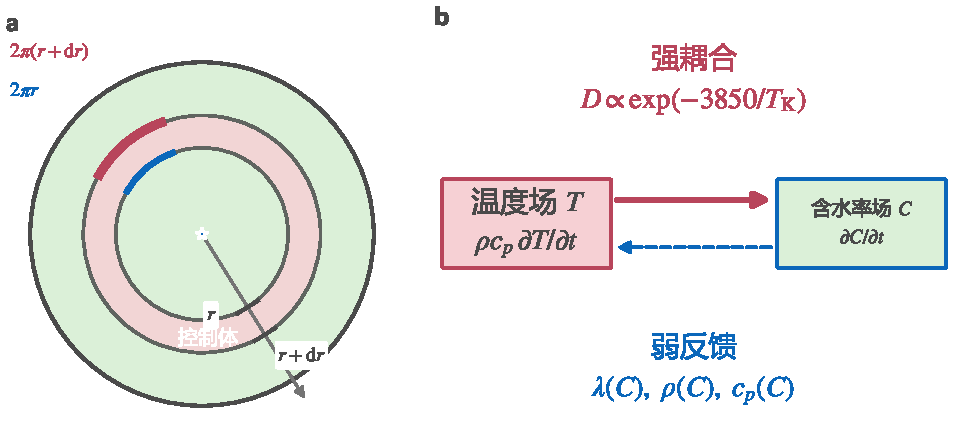
\includegraphics[width=0.9\textwidth,height=0.8\textheight,keepaspectratio]{../figures/fig_mech_coupling.pdf}
  \caption{守恒律的面积加权与双向耦合。环形控制体内外两个柱面的通过面积不
  相等，这是圆柱几何区别于平板的根源，整理后在方程中留下面积加权项；温度对
  扩散系数是强耦合，含水率对热物性只是弱反馈。}
  \label{fig:mech-coupling}
\end{figure}

左侧图示说明同样大小的通量在大半径处对应更大的通过面积，因此表面附近的浓度变化被放大而中心区被相对屏蔽；干燥总是从外向内推进，几何本身已经贡献了一部分原因。右侧则表明两个方程的耦合是不对称的：温度经 Arrhenius 因子强烈改变扩散系数，含水率只通过密度、比热容与导热系数对温度场的时间常数产生温和的反馈。这种单向强、反向弱的结构使得求解时可以把两个方程放在同一时间层内迭代，而不必担心反馈回路造成的迭代震荡。

\subsection{初始条件、边界条件与烘房激励}

初始时刻药材整体处于均匀状态，

\begin{equation}
T(r,0)=T_0=28\ ^{\circ}\mathrm{C},\qquad C(r,0)=C_0=2.55\ \mathrm{kg/kg},\qquad 0\le r\le R_0 .
\label{eq:ic}
\end{equation}

轴线处由轴对称性给出零通量，

\begin{equation}
\left.\frac{\partial T}{\partial r}\right|_{r=0}=0,\qquad
\left.\frac{\partial C}{\partial r}\right|_{r=0}=0 .
\label{eq:bc0}
\end{equation}

表面处热量与水分都以第三类边界条件与烘房交换，即内部输运到表面的通量等于表面与空气之间的对流交换量，

\begin{equation}
\left.-\lambda(C)\frac{\partial T}{\partial r}\right|_{r=R}=h\,\big[T(R,t)-T_a(t)\big],
\qquad
\left.-D(C,T)\frac{\partial C}{\partial r}\right|_{r=R}=h_m\,\big[C(R,t)-C_a(t)\big].
\label{eq:bcR}
\end{equation}

题目给出的对流换热系数 $25$~W/(m$^2\cdot$K) 与热风干燥实测的对流换热系数量级相符\upcite{akpinar2015htc}，而只给一个对流传质系数、不给相间换算关系的做法，与传热传质类比中以同一形式处理两个 Robin 条件的惯例一致\upcite{ghiaasiaan2018analogy}。选择第三类而非第一类边界并非形式偏好。以初始物性估算，传热毕奥数 ${\rm Bi}_h=hR_0/\lambda\approx1.4$，量级为一，说明表面对流阻力与内部导热阻力相当，既不能把药材当作温度均匀的集中体，也不能把表面温度直接指定为空气温度。传质一侧 ${\rm Bi}_m=h_mR_0/D$ 在初始时刻约为 $3$，随着表层变干而增大到千的量级，表明水分迁移越来越受内部扩散控制，表面对流则退化为一个次要环节。

需要强调，式~\eqref{eq:bcR} 中的 $C$ 与 $C_a$ 虽同为“水分浓度”且单位相同，却分属药材与空气两个载体，数值上相差约两个数量级，任何环节都不得把两者合并为同一个场。烘房激励 $T_a(t)$ 与 $C_a(t)$ 由实测序列线性插值给出，图~\ref{fig:oven-input} 展示了这套激励的形态及其延拓依据。

\begin{figure}[htbp]
  \centering
  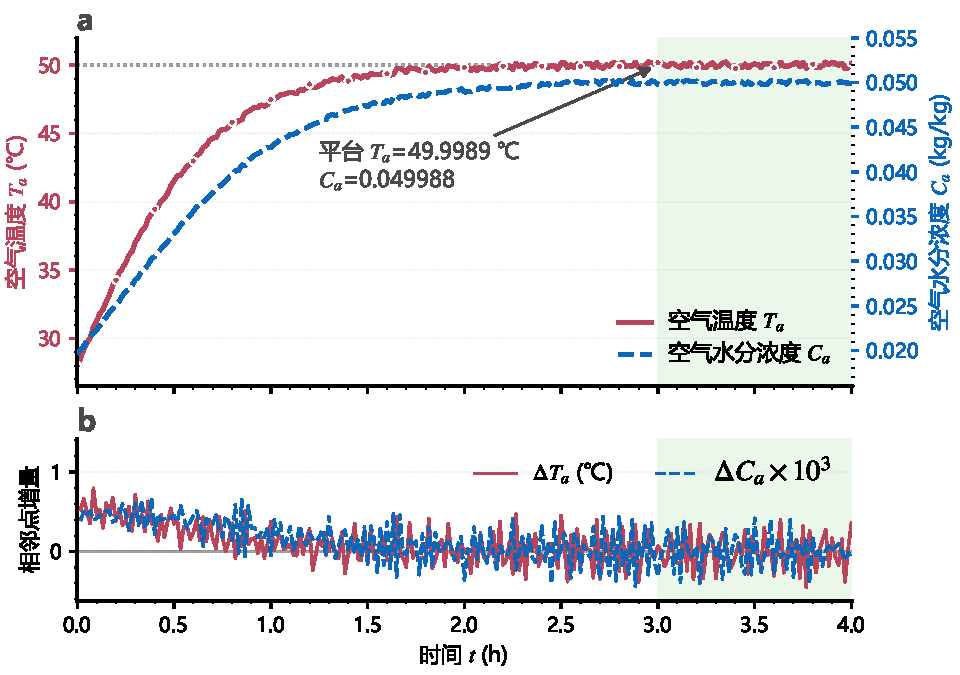
\includegraphics[width=0.9\textwidth,height=0.8\textheight,keepaspectratio]{../figures/fig_oven_input.pdf}
  \caption{附件 1 给出的烘房运行条件（241 点实测，未作平滑）。a：空气温度
  $T_a$ 先升温后维持恒定，空气水分浓度 $C_a$ 与之反向变化，两者是表面两个
  Robin 边界的驱动量；b：逐点一阶差分，末段 61 点的增量落在零线附近，据此
  判定序列已进入恒定平台，平台均值用于时间超出实测区间后的延拓。}
  \label{fig:oven-input}
\end{figure}

实测序列在四小时内把空气温度由 $28$~°C 抬到约 $50$~°C 后保持不动，空气水分浓度则由 $0.0196$~kg/kg 升到约 $0.0500$~kg/kg，两者反向变化对应加热与加湿的先后。右图的逐点差分把“是否已进入平台”变成一个可判断的问题：末段 61 个点的增量全部贴近零线，因此把该段的实测均值 $T_a=49.9989$~°C、$C_a=0.049988$~kg/kg 用作四小时之后的常值延拓，而不是对趋势作外推拟合。这样处理的代价是全程约九成的时间依赖平台假设，好处是不引入题面之外的任何参数。

\subsection{三套物性及其适用范围}

题目为三个不同情形分别给出物性经验公式，且互相排斥：预热阶段用第一套，全过程与合格时长判定用第二套，考虑收缩时用第三套；对流换热系数 $h=25$~W/(m$^2\cdot$K) 与对流传质系数 $h_m=8\times10^{-7}$~m/s 则全题通用。三套物性的具体形式为
\begin{align}
\text{附录 2：}&\ \rho=820,\quad c_p=2600,\quad \lambda=0.36,\quad D=7\times10^{-9}e^{-0.89/C};
\label{eq:app2}\\
\text{附录 3：}&\ \rho=650+128C,\quad c_p=1450+2736\tfrac{C}{C+1},\quad
\lambda=0.21+0.38\tfrac{C}{C+1},\notag\\
&\ D=2.4\times10^{-3}e^{-0.45/C}e^{-3850/T_{\rm K}};
\label{eq:app3}\\
\text{附录 4：}&\ \rho=760+90C,\quad c_p=1850+2150\tfrac{C}{C+1},\quad
\lambda=0.12+0.20\tfrac{C}{C+1},\notag\\
&\ D=4.2\times10^{-4}e^{-0.30/C}e^{-3850/T_{\rm K}} .
\label{eq:app4}
\end{align}

三套物性中扩散系数同时含有含水率因子与温度因子，这与实验测定给出的有效扩散系数形式一致：温度依赖按 Arrhenius 型给出\upcite{doymaz2016kinetics}，含水率依赖则来自内部迁移阻力随脱水而变化\upcite{yang2007internal}，两者相乘的写法在不同干燥方式的实测数据上都能成立\upcite{richter2016vacuum}。三处细节直接决定结果是否正确。其一，Arrhenius 因子中的温度必须取绝对温度，若误用摄氏读数，指数项将相差数十个数量级，干燥过程永远不会结束。其二，浓度因子的指数为 $-a/C$，含水率在分母上，因此扩散系数随药材变干而减小，这正是干燥后期表层阻力急剧增大、也就是俗称“结壳”的数学表现。其三，比热容与导热系数的自变量是湿基含水率 $C/(C{+}1)$ 而非干基含水率，初始状态下前者为 $0.7183$，若误用干基会使两项系统性偏大。图~\ref{fig:prop-curves} 把三套物性逐项画在一起。

\begin{figure}[htbp]
  \centering
  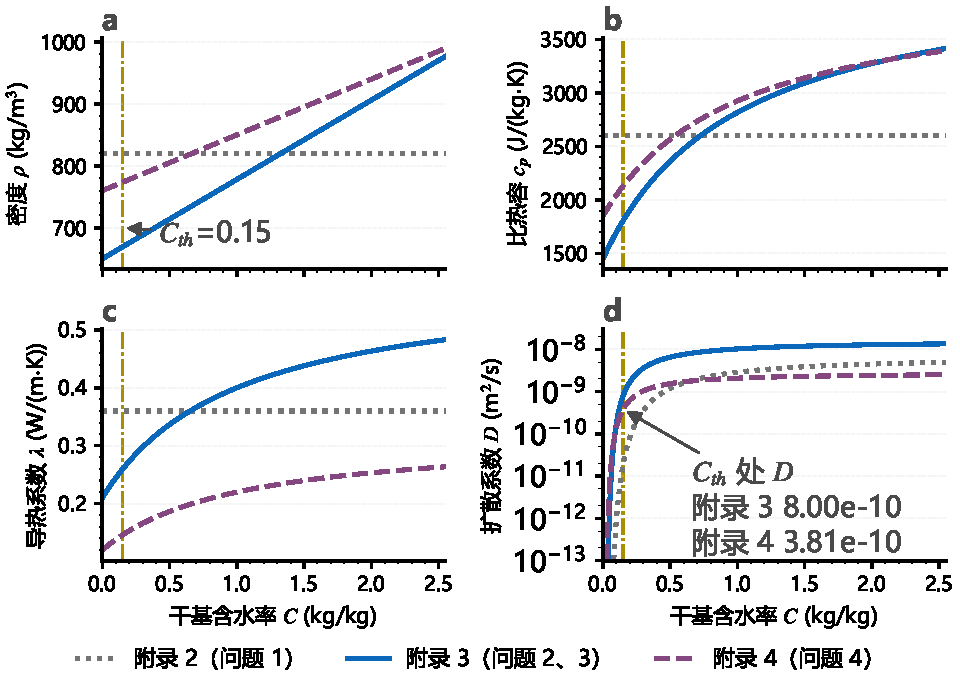
\includegraphics[width=0.9\textwidth,height=0.8\textheight,keepaspectratio]{../figures/fig_prop_curves.pdf}
  \caption{附录 2/3/4 三套物性的逐项对照，横轴为干基含水率，点划线标出判据
  阈值 $C_{th}=0.15$ 的位置。a—c：密度、比热容、导热系数；附录 2 为常物性，
  附录 3/4 随含水率变化（比热与导热按湿基 $C/(C{+}1)$ 取值）。d：扩散系数取
  对数纵轴，跨越四个数量级，是三套物性中差异最大的一项。曲线均按附录给出的
  经验公式直接计算，未作任何拟合或平滑。}
  \label{fig:prop-curves}
\end{figure}

前三幅图中，密度、比热容与导热系数在整个含水率区间内的变化都不超过一倍，其中导热系数从湿态的 $0.48$ 降到阈值附近的 $0.26$，量级始终不变。第四幅图必须用对数纵轴才能容纳：第二套物性在 $50$~°C 下，扩散系数由初始含水率处的 $1.35\times10^{-8}$~m$^2$/s 降到阈值处的 $8.0\times10^{-10}$~m$^2$/s，再降到最干处的 $2.0\times10^{-12}$~m$^2$/s，前后跨越四个数量级。这一项既是数值求解全部困难的来源，也是三套物性中差异最大的一项——第三套的前因子比第二套小了将近一个数量级。

\subsection{顶点式有限体积离散}

物性随解变化使方程为非线性，且扩散系数在空间上的刚性比可达 $10^4$，离散格式必须同时保证守恒性与稳定性。本文采用顶点式有限体积法：把归一化半径 $N$ 等分，节点取在 $s_i=i\Delta s$，$\Delta s=1/N$，控制体取相邻节点的中点连线所夹区间，两端为半控制体。选顶点式而非格心式的直接理由是题目要求的输出位置恰好落在节点上，$N=20$ 时节点即 $r=0,0.1,\dots,2.0$~cm，加密到 $N=40$ 或 $80$ 时原节点仍是子集，交付结果无需任何空间插值。控制体的无量纲体积由精确积分得到，

\begin{equation}
V_0=\frac{(\Delta s)^2}{8},\qquad
V_i=i\,(\Delta s)^2\ (1\le i\le N-1),\qquad
V_N=\frac{(\Delta s)^2}{2}\left(N-\frac14\right),
\label{eq:vol}
\end{equation}

三式合起来满足 $\sum_i V_i=1/2=\int_0^1 s\,\mathrm{d}s$，即离散域的体积与连续域严格相等。把式~\eqref{eq:mass} 在控制体上积分，散度项化为界面通量之差，得

\begin{equation}
V_i\frac{C_i^{n+1}-C_i^{n}}{\Delta t}
=\frac{1}{R^2}\left[
s_{i+\frac12}D_{i+\frac12}\frac{C_{i+1}^{n+1}-C_i^{n+1}}{\Delta s}
-s_{i-\frac12}D_{i-\frac12}\frac{C_i^{n+1}-C_{i-1}^{n+1}}{\Delta s}\right].
\label{eq:disc}
\end{equation}

两个边界都不需要虚节点。轴线一侧的界面面积因子 $s_{-1/2}=0$ 使该项自动消失，式~\eqref{eq:bc0} 的零通量条件在离散层面精确满足；表面一侧的界面就是物理表面，把式~\eqref{eq:bcR} 直接代入即贡献一项 $-h_m\big[C_N^{n+1}-C_a\big]/R$。温度方程与之同构，只需把 $V_i$ 换成 $\rho_ic_{p,i}V_i$、$D$ 换成 $\lambda$、$h_m$ 换成 $h$、$C_a$ 换成 $T_a$。图~\ref{fig:mech-fvm} 给出网格布置与由此得到的代数结构。

\begin{figure}[htbp]
  \centering
  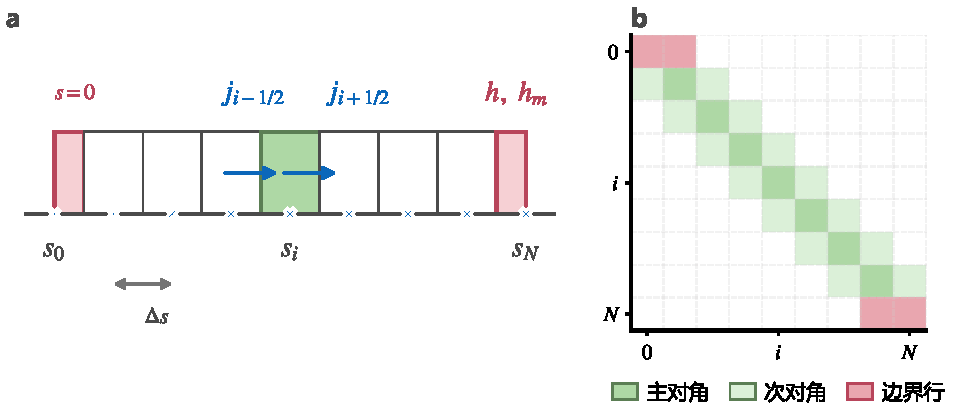
\includegraphics[width=0.9\textwidth,height=0.8\textheight,keepaspectratio]{../figures/fig_mech_fvm.pdf}
  \caption{顶点式有限体积网格与代数结构。节点落在输出要求的位置上，两端为
  半控制体；内侧界面的面积因子为零使轴线零通量精确满足，不需虚节点，由此得
  到的系数矩阵严格三对角。图中网格数仅为作图清晰，不代表实算网格。}
  \label{fig:mech-fvm}
\end{figure}

由于每个控制体只与左右两个邻居交换通量，系数矩阵严格三对角，可用追赶法在 $O(N)$ 次运算内直接求解，不引入迭代求逆的误差。时间方向采用全隐式格式：显式格式的稳定性上限为 $\Delta t\le\Delta r^2/(2D_{\max})$，本题扩散系数的空间最大值出现在湿润的中心区，在 $\Delta r=5\times10^{-4}$~m 时该上限约为 $9.3$~s，而总时长在 $2\times10^5$~s 量级，显式推进需要数万步且步长完全由稳定性而非精度决定。全隐式配合三对角直接解使时间步只受精度约束。

\subsection{界面扩散系数的取法}

式~\eqref{eq:disc} 中界面系数 $D_{i+1/2}$ 的取法在本题中不是细节。扩散系数跨越四个数量级，相邻节点上的取值可能相差十倍以上，此时常用的调和平均会被两者中的较小者支配，$D_{i+1/2}\approx2\min(D_i,D_{i+1})$。表面附近含水率梯度极陡，最外侧控制体的含水率随网格加密而不断降低，界面系数随之持续变小，形成不随网格细化而消失的偏差。实算可以直接看到这一失效：取调和平均时，$N=20,40,80$ 给出的合格时长为 $549.918$、$223.428$、$87.440$~h，网格每加倍结果几近减半，根本不收敛。

问题的根源在于调和平均的适用前提是界面两侧为分区常系数的复合介质，此时串联阻力叠加给出精确通量；而本题的 $D(C,T)$ 是含水率的光滑函数，界面两侧的差异完全由离散产生，并非物理跳变。回到通量本身即可得到正确的取法：引入 Kirchhoff 势 $\Phi(C)=\int_0^C D(c,\bar T)\,\mathrm{d}c$ 后通量写作 $j=-\partial\Phi/\partial r$，相邻节点间的精确通量为 $-(\Phi_{i+1}-\Phi_i)/\Delta r$。把它整理成式~\eqref{eq:disc} 所用的形式，界面系数只能是

\begin{equation}
D_{i+\frac12}=\frac{1}{C_{i+1}-C_i}\int_{C_i}^{C_{i+1}} D\!\left(c,\ \tfrac{T_i+T_{i+1}}{2}\right)\mathrm{d}c ,
\qquad
\lim_{C_{i+1}\to C_i}D_{i+\frac12}=D\!\left(C_i,\tfrac{T_i+T_{i+1}}{2}\right).
\label{eq:iface}
\end{equation}

该积分用八点 Gauss--Legendre 求积计算，对 $e^{-a/C}$ 型被积函数的相对误差在 $10^{-10}$ 以下；两节点含水率之差小于 $10^{-12}$ 时退化为中点取值以避免零比零。改用积分平均后，同一组网格给出的合格时长立即收敛，逐档变化只有 $0.052\%$ 与 $0.014\%$，不再有随网格漂移的趋势；三档的具体数值列于表~\ref{tab:conv}。式~\eqref{eq:iface} 在系数为常数时退化为该常数，在真实分区跳变时退化为调和平均，因此是算术平均与调和平均的共同推广，没有适用性损失。导热系数在整个区间内变化不足一倍，其界面取值方式对结果无实质影响，仍按调和平均处理。

\subsection{非线性迭代与时间步安排}

物性依赖待求解，故每个时间层内做一轮不动点迭代：以上一层解为初值，用当前迭代值计算 $\rho,c_p,\lambda,D$ 与界面系数，解两个三对角系统，直到

\begin{equation}
\max\!\Big(\big\|C^{(k+1)}-C^{(k)}\big\|_\infty,\ \ 10^{-3}\big\|T^{(k+1)}-T^{(k)}\big\|_\infty\Big)<10^{-11},
\label{eq:picard}
\end{equation}

迭代次数上限取 60。式~\eqref{eq:picard} 中温度残差乘以 $10^{-3}$ 是一个容差配比：两个场的单位不同，用同一个绝对阈值并无意义，该权因子相当于对含水率要求 $10^{-11}$~kg/kg、对温度要求 $10^{-8}$~°C。含水率一侧收得更紧是因为停时判据直接由含水率定义，而 $10^{-8}$~°C 的温度残差已远低于任何有物理意义的分辨率。实算表明恒温平台段三到五次迭代即收敛，预热段峰值为 12 次。

时间步按阶段分段：$1800$~s 以内取 $0.01$~s 以分辨升温初期最陡的瞬变，$1800$ 至 $14400$~s 取 $1$~s 覆盖实测激励段，其后取 $60$~s 与后续输出间隔一致。各问的输出间隔按题面要求另行设定（问题一、二每 $1$~s，问题三、四每 $60$~s），都是相应步长的整数倍，逐秒输出的要求由此自动满足。平台段的步长收敛性经实算确认：$\Delta t$ 由 $120$~s 依次细化到 $60$、$30$、$10$~s，合格时长的逐档相对变化为 $0.081\%$、$0.041\%$、$0.027\%$，$60$~s 相对 $10$~s 的偏差为 $0.068\%$，已远小于结果的有效位数需求，因此取 $60$~s 作为生产设置；四档数值同见表~\ref{tab:conv}。
